%!TEX root = ../dissertation.tex

\chapter{Methodology}
\label{methodology}

\section{Approach}

\begin{figure}[ht]
	\centering
	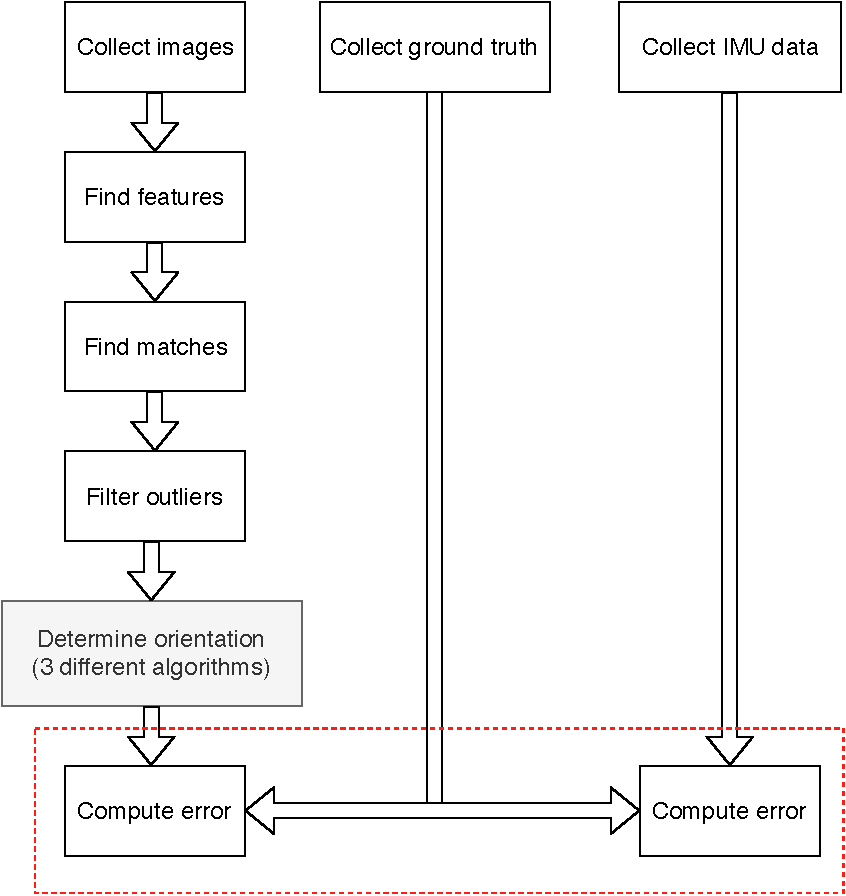
\includegraphics[width=0.7\textwidth]{images/approach.pdf}
	\caption[Approach Diagram]{Approach Diagram. Using the \acrshort{rgb} camera, two images are collected, before and after rotation. In each image, features are detected and matched between them. Some matches might be false or have too much noise, so they are filtered out. Using the matches information, the orientation is determined using an estimation algorithm. 3 algorithms will be put to test. Finally, the orientation determined is compared against the ground truth. The \acrshort{imu}'s orientation output is also compared against the ground truth to evaluate the improvement in relation to the camera.}
	\label{cha3:methodology:approach}
\end{figure}


\subsection{Feature detection and matching}

\subsection{Filtering matches}

\subsection{Determine orientation}

\subsubsection{Translation derivation}

As mentioned before, because the current eye prototype is a coupled system, the translation can be obtained with the knowledge of the rotation and the baseline length. This length is defined as the distance from the center of the camera sensor to the center of rotation, as shown on Figure
\ref{cha3:detori:translation}.

\begin{figure}[ht]
	\centering
	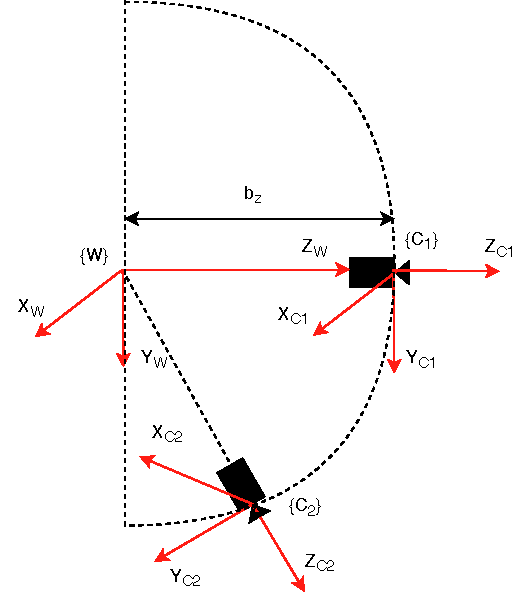
\includegraphics[width=0.5\textwidth]{images/transf.pdf}
	\caption[Translation derivation]{Translation derivation. Effect of a rotation on the current eye prototype's coupled system. The rotation and the baseline length define the translation. ${W}$ is the world reference frame centered on the rotation center, ${C_1}$ is the reference frame of the camera in the first position and ${C_2}$ is its frame on the second position, after rotating. $b_z$ is the baseline length on the Z axis.}
	\label{cha3:detori:translation}
\end{figure}

The translation can be easily derived as follows using . Having the world reference frame, ${W}$, set at the center of rotation, the transformation from the world to the first position of the camera, ${C_1}$, is

\begin{equation}
^W_{C_1}T = \begin{bmatrix}
I & -\mathbf{b}\\ 
\mathbf{0} & 1
\end{bmatrix},
\end{equation} 

where $I$ is the identity matrix and $\bf b$ is the baseline length expressed in each axis, $X$, $Y$ and $Z$, as $\mathbf{b} = [b_X \ b_Y \ b_Z]$. 

The transformation from the world reference frame to the second position of the camera, ${C_2}$, is
\begin{equation}
^W_{C_2}T = \begin{bmatrix}
R & -\mathbf{b}\\ 
\mathbf{0} & 1
\end{bmatrix},
\end{equation}\\
where $R$ is the rotation.

Hence, the transformation from the first position of the camera to the second can be obtained as
\begin{equation}
^{C_1}_{C_2}T = ^{W}_{C_2}T ^{C_1}_{W}T = ^{W}_{C_2}T ^{W}_{C_1}T^{-1} = 
\begin{bmatrix}
R & -\mathbf{b}\\ 
\mathbf{0} & 1
\end{bmatrix}
\begin{bmatrix}
I & \mathbf{b}\\ 
\mathbf{0} & 1
\end{bmatrix}
=
\begin{bmatrix}
R & R\mathbf{b}-\mathbf{b}\\ 
\mathbf{0} & 1
\end{bmatrix}.
\end{equation}
And finally, the translation ends up as
\begin{equation}
\mathbf{t}(R, \mathbf{b}) = R\mathbf{b}-\mathbf{b} = (R-I)\mathbf{b}.
\end{equation}


\subsubsection{\acrlong{grat}}

por isto no background
SAY THAT EPIPOLAR IS GOOD CUZ NO NEED TO DETERMINE Z, reference PAMI paper
IN TERMS OF R INSTEAD OF F
\subsubsection{\acrlong{mbpe}}
\label{MBaPE}
This method is a bundle adjustment of the previous one. It uses the rotation matrix obtained with OPPr and it tries to tune it to obtain a rotation and a translation dependent on the former, through 
\begin{align*}
	& \min_{R, Z_{e11}, ..., Z_{e1N}} \sum^N_{i=1} [(u_{e1i}-u_{1i})^2 + (u_{e2i}-u_{2i})^2 + (v_{e1i}-v_{1i})^2 + (v_{e2i}-v_{2i})^2]\\
	& \text{with} \ Z_{e1init} = \frac{1}{\sqrt{u_{1i}^2 + v_{1i}^2 + 1}} \ \text{and} \ R_{init} = R_{oppr},
\end{align*}
where $u_{1i}$ and $v_{1i}$ are the image points of the Camera View 1, $u_{2i}$ and $v_{2i}$ are the image points of the Camera View 2, $u_{e1i}$, $v_{e1i}$, $u_{e2i}$ and $v_{e2i}$ are the corresponding image points estimations and $Z_{e1i}$ is the depth of the Camera View 1.\\
The image point estimations are obtained the following way
\begin{align*}
	\mathbf{m_{e1}} = \frac{KR^T(Z_{e2}K^{-1}\mathbf{m_2}) - R^Tt)}{Z_{e1}}\\
	\mathbf{m_{e2}} = \frac{KR(Z_{e1}K^{-1}\mathbf{m_1}) + t)}{Z_{e2}}.
\end{align*} The depth is initialized by projecting the image points in a sphere.

\subsection{Simulator}

\subsection{Real world}

\subsubsection{Ground Truth}

\subsection{C++ Library}